%!TEX program = xelatex
\documentclass[a4paper, 12pt, UTF8]{ctexart}
\usepackage[english]{babel}
\usepackage[utf8]{inputenc}
\usepackage{johd}
\usepackage{ctex} % 支持中文
\usepackage{amsmath}
\usepackage{graphicx}
\usepackage{caption}
\usepackage{subcaption} 
\usepackage{amssymb}
\newcommand{\bs}[1]{\boldsymbol{#1}}


\title{空气动力学方程组间断有限元方法}

\date{} %leave blank

\begin{document}

\maketitle


\section{方程简介}
考虑二维Euler方程组,将其写成双曲守恒律形式:
\begin{equation}
 \begin{cases}
    	\bs {u_{t}}+\nabla \cdot \bs f(\bs u)=0 \\
    	\bs u(x, y, 0)=\bs{u_{0}}(x, y)
    \end{cases} \quad (x, y, t)  \in \Omega \times(0, T)
\end{equation}
其中,$\bs u$为守恒量,$\bs f(u)=\left(f_{1}(u), f_{2}(u)\right)$ 为通量,
\begin{equation}
\bs{u}=\begin{bmatrix}
	u_0\\
	u_{1}\\
	u_{2}\\
	 u_3
\end{bmatrix}
=\begin{bmatrix}
	\rho\\
	\rho v_{1}\\
	\rho v_{2}\\
	 E
\end{bmatrix}
\quad f_{1}(\bs{u})=\begin{bmatrix}
	\rho v_{1}\\
	\rho v_{1}^{2}+p\\
	\rho v_{1} v_{2}\\
	(E+p) v_{1}
\end{bmatrix},\quad
f_{2}(\bs{u})=\begin{bmatrix}
	\rho v_{2}\\
	 \rho v_{1} v_{2}\\
	 \rho v_{2}^{2}+p\\
	 (E+p) v_{2}
\end{bmatrix}
\end{equation}
其中, $\rho$ 表示密度,$v_{1}$ 为$x$方向的速度,$v_{2}$ 为$y$方向的速度,E为能量,压力 
\begin{equation}\label{pressure}
p=(\gamma-1)\left(E-\frac{1}{2} \rho\left(v_{1}^{2}+v_{2}^{2}\right)\right)=(\gamma-1)\left(u_3-\frac{1}{2u_0} \left(u_1^{2}+u_{2}^{2}\right)\right)
\end{equation}
绝热指数 $\gamma$在计算中一般取为常数1.4。

下面给出二维Euler方程的一个有光滑解的例子,常用来测试算法的精度。在该例子中,计算区域$\Omega=[0,2] \times[0,2]$,给定 
初始条件: 
\begin{equation}
\begin{cases}
	   \rho(x, y, 0)=1+0.2 \sin (\pi(x+y)) \\
	   v_{1}(x, y, 0)=0.7, \quad v_{2}(x, y, 0)=0.3  \\
	   p(x, y, 0)=1 
    \end{cases}
\end{equation}
取周期边界条件, 则密度函数有精确解:
$$\rho(x, y, t)=1+0.2 \sin (\pi(x+y-t))$$
该算例一般可以计算到$T = 2$。




\section{基函数与外法向量}
设$\mathcal T_h=\{K\}$为区域$\Omega$的一个三角形剖分,在$\mathcal T_h$中的任意一个三角形$K$上, 设$\{(x_i, y_i)\}_{i=0}^2$为三角形的三个顶点的坐标,且顶点顺序按逆时针方向排列,如图\ref{triangle}所示。三角形三个顶点所对的三条边的中点分别记为$m_{i}=\left(\hat{x}_{i}^K, \hat{y}_{i}^K\right)$,$i=0, 1, 2$,其中$m_i$为第$i$个顶点所对的
边的中点,即
\begin{equation}
\begin{split}
\hat x_0^K=\frac{x_1^K+x_2^K}{2},\quad  \hat x_1^K=\frac{x_0^K+x_2^K}{2},\quad\hat x_2^K=\frac{x_0^K+x_1^K}{2},\\
 \hat y_0^K=\frac{y_1^K+y_2^K}{2},\quad\hat y_1^K=\frac{y_0^K+y_2^K}{2},\quad  \hat y_2^K=\frac{y_0^K+y_1^K}{2}.
\end{split}
\end{equation}
如图\ref{triangle}所示。定义三个基函数
\begin{equation}
\begin{split}
\displaystyle \varphi_{0}^K(x, y)=\frac{\left(\hat{y}_{1}^K-\hat{y}_{2}^K\right)\left(x-\hat{x}_{1}^K\right)+\left(\hat{x}_{2}^K-\hat{x}_{1}^K\right)\left(y-\hat{y}_{1}^K\right)}{\left(\hat{y}_{1}^K-\hat{y}_{2}^K\right)\left(\hat{x}_{0}^K-\hat{x}_{1}^K\right)+\left(\hat{x}_{2}^K-\hat{x}_{1}^K\right)\left(\hat{y}_{0}^K-\hat{y}_{1}^K\right)}\\
 \varphi_{1}^K(x, y)=\frac{\left(\hat{y}_{2}^K-\hat{y}_{0}^K\right)\left(x-\hat{x}^K_{2}\right)+\left(\hat{x}^K_{0}-\hat{x}_{2}^K\right)\left(y-\hat{y}^K_{2}\right)}{\left(\hat{y}_{2}^K-\hat{y}_{0}^K\right)\left(\hat{x}_{1}^K-\hat{x}_{2}^K\right)+\left(\hat{x}_{0}^K-\hat{x}^K_{2}\right)\left(\hat{y}_{1}^K-\hat{y}_{2}^K\right)}\\
 \varphi_{2}^K(x, y)=\frac{\left(\hat{y}_{0}^K-\hat{y}_{1}^K\right)\left(x-\hat{x}^K_{0}\right)+\left(\hat{x}_{1}^K-\hat{x}^K_{0}\right)\left(y-\hat{y}_{0}^K\right)}{\left(\hat{y}_{0}^K-\hat{y}_{1}^K\right)\left(\hat{x}_{2}^K-\hat{x}_{0}^K\right)+\left(\hat{x}_{1}^K-\hat{x}_{0}^K\right)\left(\hat{y}_{2}^K-\hat{y}_{0}^K\right)}
\end{split}
\end{equation}
显然,它们满足
\begin{equation}
\varphi_{i}^K(\hat{x}_{j}^K, \hat{y}_{j}^K)=\delta_{ij}=\begin{cases}
\displaystyle 0,\quad i\neq j\\
\displaystyle 1, \quad i=j
\end{cases}
\end{equation}
利用这些基函数, 我们可以在$K$上定义$\bs u$的近似
\begin{equation}\label{numericsolution}
\bs u_{h}^K(x, y, t)=\sum\limits_{i=0}^{2} \bs u_{i}^K(t) \varphi_{i}^K(x, y) \quad(x, y) \in K
\end{equation}
\begin{figure}[!ht]
\centering
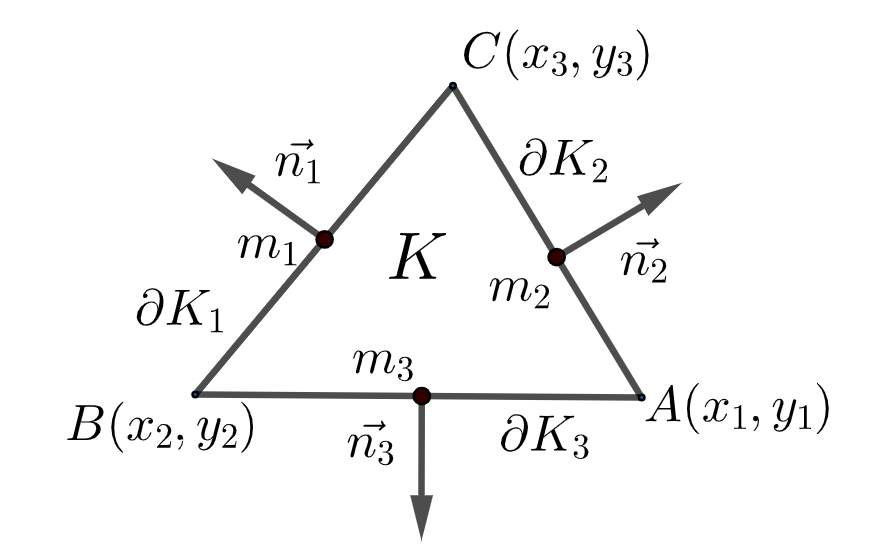
\includegraphics[width=0.5\textwidth]{images/1.png}
\caption{三角形单元}
\label{triangle}
\end{figure}

\newpage

通过计算可知,基函数 $\left\{\varphi_{i}^K(x, y)\right\}_{i=0}^2$ 满足:
\begin{equation}\label{othorgnal}
\int_{K} \varphi_{i}^K(x, y) \varphi_{j}^K(x, y) d x d y=
\begin{cases}
\displaystyle 	0, \quad i \neq j \quad(\text { 相互正交) } \\
\displaystyle 	\frac{|K|}{3} \sum\limits_{m=1}^{3} (\varphi_{j}^K)^{2}\left(\hat{x}_{m}^K, \hat{y}_{m}^K\right)=\frac{|K|}{3}, \quad i=j   
    \end{cases}
\end{equation}
其中 
$$|K|=\frac{1}{2}\left|\begin{array}{lll}
1 & x_{0}^K & y_{0}^K\\
1 & x_{1}^K & y_{1}^K \\
1 & x_{2}^K & y_{2}^K 
\end{array}\right| = \frac{1}{2}\left| x_{0}^K\left(y_{1}^K-y_{2}^K\right)+x_{1}^K\left(y_{2}^K-y_{0}^K\right)+x_{2}^K\left(y_{0}^K-y^K_{1}\right)\right|$$ 为三角形$K$的面积。

通过变换
\begin{equation}
\begin{cases}
\displaystyle x=x(\xi,\eta)=x_0\xi+x_1\eta+x_2(1-\xi-\eta)\\
\displaystyle y=y(\xi,\eta)=y_0\xi+y_1\eta+y_2(1-\xi-\eta)
\end{cases}
\end{equation}
可将三角形$K$变换到标准三角形单元$\widehat K=\{(\xi, \eta)| \xi+\eta\leq 1, 0\leq \xi,\eta \leq 1\}$,那么基函数在参考坐标$\xi,\eta$下的表达式为
\begin{equation}
\begin{split}
	\hat\varphi_0(\xi,\eta)=&\varphi_0^K(x(\xi,\eta),y(\xi,\eta))=1-2\xi, \quad \hat\varphi_1(\xi,\eta)=\varphi_1^K(x(\xi,\eta),y(\xi,\eta))=1-2\eta,\\ \hat\varphi_2(\xi,\eta)=&\varphi_2^K(x(\xi,\eta),y(\xi,\eta))=2\xi+2\eta-1.
\end{split}
\end{equation}
利用变换将$K$上的积分转换到参考单元上得
\begin{equation}\label{transformedintegral}
\int_K\varphi_i^K(x, y)\varphi_j^K(x, y)dxdy=2|K|\int_0^1\int_{0}^{1-\xi}\hat\varphi_i(\xi,\eta)\hat\varphi_j(\xi,\eta)d\eta d\xi
\end{equation}
经过简单计算我们有
\begin{equation}
\int_0^1\int_{0}^{1-\xi}\hat\varphi_0(\xi,\eta)\hat\varphi_0(\xi,\eta)d\eta d\xi =\frac{1}{6},\quad \int_0^1\int_{0}^{1-\xi}\hat\varphi_0(\xi,\eta)\hat\varphi_1(\xi,\eta)d\eta d\xi =0.
\end{equation}
类似我们还可以验证得
\begin{equation}
\int_0^1\int_{0}^{1-\xi}\hat\varphi_i(\xi,\eta)\hat\varphi_j(\xi,\eta)d\eta d\xi =\begin{cases}
\displaystyle\frac{1}{6},\quad i=j\\
\displaystyle 0,\quad i\neq j
\end{cases}
\end{equation}
将上述结论代入\eqref{transformedintegral}可得\eqref{othorgnal}。


设$\bs n_{0}$, $\bs n_{1}$,$\bs n_{2}$ 分别表示为单元$K$三个顶点所对的边上的单位外法向量,如图 \ref{triangle} 所示。如果顶点$A(x_0^K, y_0^K)$,$B(x_1^K, y_1^K)$,$C(x_2^K, y_2^K)$按逆时针方向排列,则有:
\begin{equation}
\begin{split}
\bs{B C}=\left(x_{2}^K-x_{1}^K, y_{2}^K-y_{1}^K\right),\quad \bs{n_{0}}=\left(y_{2}^K-y_{1}^K, x_{1}^K-x_{2}^K\right) /|BC|\\
\bs{C A}=\left(x_{0}^K-x_{2}^K, y_{0}^K-y_{2}^K\right),\quad \bs{n_{1}}=\left(y_{0}^K-y_{2}^K, x_{2}^K-x_{0}^K\right) /|CA|\\
\bs{A B}=\left(x_{1}^K-x_{0}^K, y_{1}^K-y_{0}^K\right), \quad \bs{n_{2}}=\left(y_{1}^K-y_{0}^K, x_{0}^K-x_{1}^K\right) /|AB|
\end{split}
\end{equation}

\newpage

\section{DG格式的空间离散}

为了求得在任意三角形单元$K$上的近似解  
\begin{equation}\label{spacediscritization}
\bs u^K_{h}(x, y, t)=\sum\limits_{i=0}^{2} \bs u^K_{j}(t) \varphi_{j}^K(x, y)
\end{equation}
我们要求近似解$\bs u^K_h(x, y, t)$在$K$上满足方程
\begin{equation}
\int_K\frac{d}{d t} \bs u_{h}^K(x, y, t)\varphi_j^Kdxdy=\int_K\bs f(\bs u_{h}^K(x, y, t))\cdot\nabla\varphi_j^Kdxdy-\int_{\partial K}\hat{\bs f}(x, y, t)\varphi_j^Kds
\end{equation}
其中$j=0, 1, 2$,$\hat{\bs f}(x, y, t)$为人为定义的数值通量,将在后面给出具体的定义。

 将表达式\eqref{numericsolution}代入上式,并应用性质\eqref{othorgnal}得,系数$\bs u_{j}^K(t)$ 满足常微分方程组:
\begin{equation}\label{semidiscrete}
 \frac{d}{d t} \bs u_{j}^K(t)=\frac{1}{\omega_{j}}\left[\int_{K} {\bs f}\left(\bs u_{h}^K(x, y, t)\right) \cdot \nabla \varphi_{j}^Kd x d y\right. \left.-\int_{\partial K}\hat{\bs f}\left(x, y, t\right) \varphi_{j}^K d s\right] 
\end{equation}
其中,$\omega_{j}=\int_{K} (\varphi_{j}^K(x, y))^2 d x d y=\frac{|K|}{3}$

方程右端的积分项可以用数值求积公式来进行计算:
\begin{equation}
\begin{split}
\int_{K} \bs f\left(\bs u_{h}^K(x, y, t)\right) \cdot  \nabla \varphi_{j}^K(x, y) &d x d y 
\approx |K| \sum_{m=0}^{2} \frac{1}{3} \bs f\left(\bs u_{h}^K\left(\hat{x}_{m}^K, \hat{y}_{m}^K, t\right)\right) \cdot \nabla \varphi_{j}^K\left(\hat{x}_{m}^K, \hat{y}_{m}^K\right)\\
=&|K| \sum_{m=0}^{2} \frac{1}{3} \bs f\left(\bs{u}^K_{m}(t)\right) \cdot \nabla \varphi_{j}^K\left(\hat{x}_{m}^K, \hat{y}_{m}^K\right)\\
\int_{\partial K}\hat{\bs f}\left(x, y, t\right) \varphi_{j}^K(x, y) d s
=&\sum_{i=0}^{2} \int_{\partial K_{i}}\hat{\bs f}(x, y, t)\varphi_{j}^K(x, y) d s \\
\approx& \sum_{i=0}^{2}\left(\left|\partial K_{i}\right| \sum_{m=0}^{1} \frac{1}{2} \hat{\bs f}\left(\bar{x}_{m}^{\partial K_i}, \bar{y}_{m}^{\partial K_i}, t\right)\varphi_{j}^K\left(\bar{x}_{m}^{\partial K_i}, \bar{y}_{m}^{\partial K_i}\right)\right)
\end{split}
\end{equation}
其中 
\begin{equation}
\begin{split}
\left(\bar{x}_{0}^{\partial K_i}, \bar{y}_{0}^{\partial K_i}\right)=\left(\hat{x}_{i}^K-\frac{\Delta x_{i}^K}{2\sqrt{3}},
 \hat{y}_{i}^K-\frac{\Delta y_{i}^K}{2\sqrt{3}} \right) \\
  \left(\bar{x}_{1}^{\partial K_i}, \bar{y}_{1}^{\partial K_i} \right)=\left(\hat{x}_{i}^K+\frac{\Delta x_{i}^K}{2\sqrt{3}} ,\hat{y}_{i}^K+\frac{\Delta y_{i}^K}{2\sqrt{3}}\right)\\
 \Delta x_{0}^K=x_{2}^K-x_{1}^K ,\quad \Delta y_{0}^K=y_{2}^K-y_{1}^K,\\  \Delta x_{1}^K=x_{0}^K-x_{2}^K ,\quad \Delta y_{1}^K=y_{0}^K-y_{2}^K,\\
  \Delta x_{2}^K=x_{1}^K-x_{0}^K ,\quad \Delta y_{2}^K=y_{1}^K-y_{0}^K.
    \end{split}
\end{equation}
 为边$\partial K_i$上的高斯求积节点,$|\partial K_{i}|$表示边的长度,如图\ref{gaussianpoint}。

\newpage
    

定义数值通量
\begin{equation}
\hat{\bs f}(x, y, t)=\hat{\bs f}\left({\bs u_{h}^{K}\left(x, y, t\right)}, {\bs u_{h}^{K'}\left(x, y, t\right)}\right)
\end{equation}
 表示在单元边界点 $(x,y)$ 处的数值通量。如图\ref{solutionlimit}所示,$\bs u_{h}^{K}\left(x, y, t\right)$ 与 $\bs u_{h}^{K'}\left(x, y, t\right)$ 分别表示单元$K$与$K'$上的数值解在$(x,y)$处的取值。
 
 \begin{figure}[h]
 \centering
 \begin{minipage}[b]{0.45\textwidth}
     \centering
     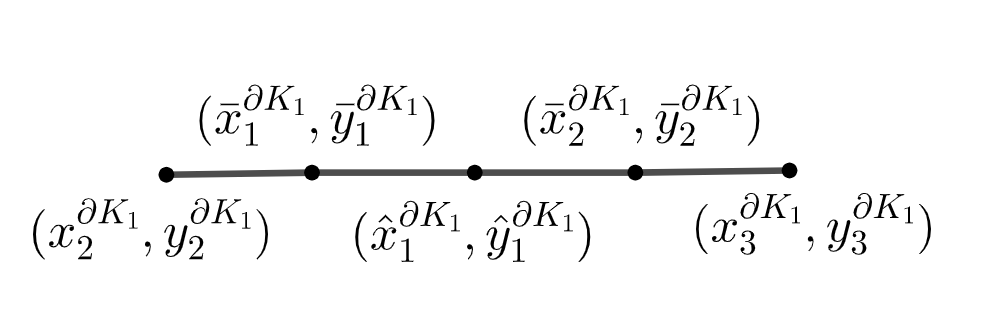
\includegraphics[width=\textwidth]{images/4.png}
     \caption{边界$\partial K_{1}$上的高斯积分点}
     \label{gaussianpoint}
 \end{minipage}
 \hspace{0.05\textwidth}
 \begin{minipage}[b]{0.45\textwidth}
     \centering
     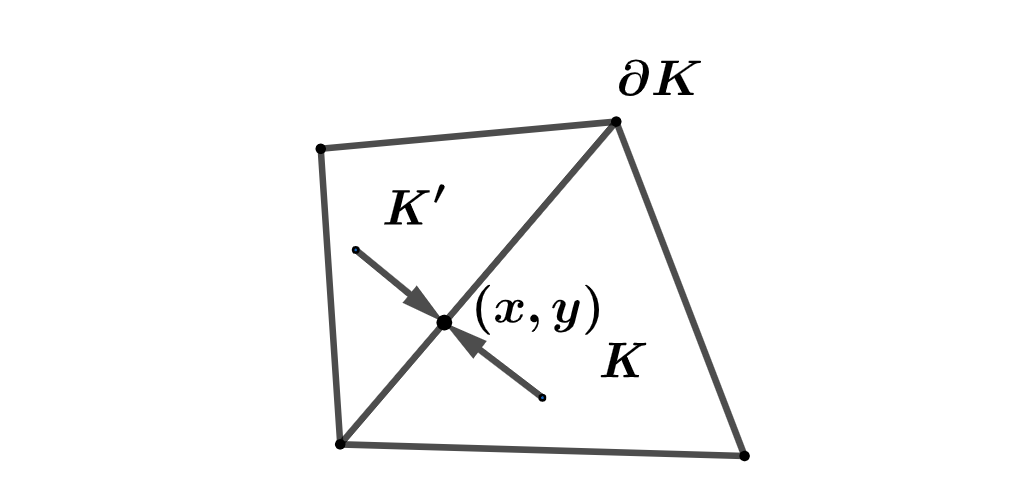
\includegraphics[width=\textwidth]{images/5.png}
     \caption{数值解在边界处的左右极限}
     \label{solutionlimit}
 \end{minipage}
 \end{figure}
 
 实际计算中,常用 $LF$ 通量:
\begin{equation}
\hat{\bs f}(x, y, t)=\frac{1}{2}\left[\bs f({\bs u_{h}^{K}\left(x, y, t\right)}) \cdot \bs{n}+\bs f({\bs u_{h}^{K'}\left(x, y, t\right)}) \cdot \bs{n}-{\alpha_{K}(x, y, t)({\bs u_{h}^{K'}\left(x, y, t\right)}-{\bs u_{h}^{K}\left(x, y, t\right)})}\right]
\end{equation}
其中$\bs{n}=\left(n_{x}, n_{y}\right)$ 表示在三角形单元K的边上的单位外法向量
\begin{equation}\label{parameteralpha}
\alpha_{K}(x, y, t)=\max \left\{\lambda\left({\bs u}_{h}^K(x, y, t)\right), \lambda\left({\bs u}_h^{K'}(x, y, t)\right)\right\}\\
\end{equation}
 $\lambda\left(\bs{u}\right)$为 $\displaystyle \frac{\partial (f(\bs{u})\cdot \bs{n})}{\partial \bs{u}} $ 的谱半径,
Jacobian矩阵定义为
\begin{equation}
	\displaystyle \frac{\partial (\bs f(\bs{u})\cdot \bs{n})}{\partial \bs{u}} =n_x\frac{\partial f_1(\bs{u})}{\partial \bs{u}}+n_y\frac{\partial f_2(\bs{u})}{\partial \bs{u}}
\end{equation}
其中
\begin{equation}
\begin{split}
		\frac{\partial f_1(\bs{u})}{\partial \bs{u}}=&\begin{bmatrix}
		\frac{\partial(\rho v_1)}{\partial\rho} & \frac{\partial(\rho v_1)}{\partial(\rho v_1)} & \frac{\partial(\rho v_1)}{\partial(\rho v_2)}& \frac{\partial(\rho v_1)}{\partial E}\\
		\frac{\partial(\rho v_1^2+p)}{\partial\rho} & \frac{\partial(\rho v_1^2+p)}{\partial(\rho v_1)} & \frac{\partial(\rho v_1^2+p)}{\partial(\rho v_2)}& \frac{\partial(\rho v_1^2+p)}{\partial E}\\
		\frac{\partial(\rho v_1v_2)}{\partial\rho} & \frac{\partial(\rho v_1v_2)}{\partial(\rho v_1)} & \frac{\partial(\rho v_1v_2)}{\partial(\rho v_2)}& \frac{\partial(\rho v_1v_2)}{\partial E}\\
		\frac{\partial((E+p) v_1)}{\partial\rho} & \frac{\partial((E+p)  v_1)}{\partial(\rho v_1)} & \frac{\partial((E+p) v_1)}{\partial(\rho v_2)}& \frac{\partial((E+p)  v_1)}{\partial E}
	\end{bmatrix}\\
	\frac{\partial f_2(\bs{u})}{\partial \bs{u}}=&\begin{bmatrix}
		\frac{\partial(\rho v_2)}{\partial\rho} & \frac{\partial(\rho v_2)}{\partial(\rho v_1)} & \frac{\partial(\rho v_2)}{\partial(\rho v_2)}& \frac{\partial(\rho v_2)}{\partial E}\\
		\frac{\partial(\rho v_1v_2)}{\partial\rho} & \frac{\partial(\rho v_1v_2)}{\partial(\rho v_1)} & \frac{\partial(\rho v_1v_2)}{\partial(\rho v_2)}& \frac{\partial(\rho v_1v_2)}{\partial E}\\
		\frac{\partial(\rho v_2^2+p)}{\partial\rho} & \frac{\partial(\rho v_2^2+p)}{\partial(\rho v_1)} & \frac{\partial(\rho v_2^2+p)}{\partial(\rho v_2)}& \frac{\partial(\rho v_2^2+p)}{\partial E}\\
		\frac{\partial((E+p) v_2)}{\partial\rho} & \frac{\partial((E+p)  v_2)}{\partial(\rho v_1)} & \frac{\partial((E+p) v_2)}{\partial(\rho v_2)}& \frac{\partial((E+p)  v_2)}{\partial E}
	\end{bmatrix}
\end{split}
\end{equation}
通过计算可得它的谱半径为:
\begin{equation}\label{spectralradius}
{\lambda}(\bs{u})=|\bs{v} \cdot \bs{n}|+c_{s}=\Big|\frac{u_1}{u_0}n_x+\frac{u_2}{u_0}n_y\Big|+c_s
\end{equation}
其中$\displaystyle c_{s}=\sqrt{\frac{\gamma{p}}{\rho}}$为声速。


\newpage

\section{时间离散}
关于系数函数$\bs u_{j}^K(t), \forall K\in\mathcal T_h, j=0, 1, 2$的常微分方程组\eqref{semidiscrete}可以将其简写为:
\begin{equation}\label{semidiscretescheme}
\frac{d \bs u_{j}^K(t)}{d t}=\bs L_{j}^K\big(\bs{u}_{h}^K(x, y, t), \bs{u}_{h}^{K'}(x, y, t), \bs{\beta}_{h}(x, y, t)\big) \quad j=0,1,2 \quad \forall K\in\mathcal T_h
\end{equation}
其中,
\begin{equation}
\begin{split}
&\bs L_{j}^K\left(\bs u_{h}^{K}(x, y, t), \bs u_{h}^{K'}(x, y, t),\bs{\beta}_{h}(x, y, t)\right)\\
= &\frac{|K|}{3\omega_j}\sum_{m=0}^{2}  \bs f\left(\bs{u}^{K}_{m}(t)\right) \cdot \nabla \varphi_{j}^K\left(\hat{x}_{m}^K, \hat{y}_{m}^K\right)\\
- &\sum_{i=0}^{2}\frac{\left|\partial K_{i}\right| }{2\omega_j}\sum_{m=0}^{1} \hat{\bs f}\left(\bar{x}_{m}^{\partial K_i}, \bar{y}_{m}^{\partial K_i}, t\right)\varphi_{j}^K\left(\bar{x}_{m}^{\partial K_i}, \bar{y}_{m}^{\partial K_i}\right)
\end{split}
\end{equation}
$\bs{\beta}_{h}(x, y, t)$ 表示数值解在计算区域的边界 $\partial \Omega$上的取值,由具体的边界条件给出,在紧邻边界的网格上计算数值通量时需要用到。

将要计算的时间区间$[0, T]$划分成剖分$0=t^0<t^1<\cdots<t^n<\cdots<t^N=T$,记$\bs u_j^{K, n}$为系数函数$\bs u_j^K(t)$在任意$t^n$时刻的近似,结合空间离散近似\eqref{spacediscritization}可得在$t^n$时刻解$\bs u(x, y, t)$在单元$K$上的全离散近似为
\begin{equation}
\bs u(x, y, t^n)\approx \sum\limits_{j=0}^2\bs u_j^{K, n}\varphi_j(x, y)
\end{equation}
为了求得所有的系数$\bs u_j^{K, n}$,我们采用二阶TVD Runge-kutta方法进行离散常微分方程组\eqref{semidiscretescheme},记第$n$步的时间步长$\Delta t^n=t^{n+1}-t^n$,那么$\bs u_j^{K, n}$的计算格式为
\begin{equation}
\begin{cases}
\displaystyle	   \bs u_{j}^{K,n+\frac{1}{2}}=\bs u_{j}^{K,n}+\Delta t^{n}\bs L_{j}^K\left(\bs u_{h}^{K, n}, \bs u_{h}^{K', n},\bs \beta_{h}\left(t^{n}\right)\right) \quad j=0,1,2 \\
\displaystyle	   \bs u_{j}^{K,n+1}=\frac{1}{2}\left(\bs u_{j}^{K, n}+\bs u_{j}^{K,n+\frac{1}{2}}\right)+\frac{1}{2} \Delta t^{n}\bs L_{j}^K\left(\bs u_{h}^{K, n+\frac{1}{2}}, \bs u_{h}^{K', n+\frac{1}{2}},\bs \beta_{h}\left(t^{n+1}\right)\right)
\end{cases}
\end{equation}
在上述推进计算中需给初始值 $\bs u_{j}^{K,0}$, 根据初始条件$\bs{u}(x, y, t=0)= \bs u_{0}(x, y)$,可设定初始值
\begin{equation}
\bs u_{j}^{K, 0}=\bs u_{0}^{K}\left(\hat{x}_{j}^K, \hat{y}_{j}^K\right) \quad j=0,1,2
\end{equation}
其中 $\left(\hat{x}_{j}^K, \hat{y}_{j}^K\right)$ 表示单元$K$第$j$号顶点所对边的中点。由于使用的是时间显格式,时间步长 $\Delta t^{n}=t^{n+1}-t^{n}$需满足限制条件
\begin{equation}
\displaystyle \Delta t^{n}=\frac{C F L}{\max\limits_{K \in \mathcal T_{h}}\Big[(\|\bs v\|+c_{s}) \cdot \frac{\text { perimeter }(K)}{|K|}\Big]}
\end{equation}
其中,$ \displaystyle \frac{\text { perimeter }(K)}{|K|}$ 为三角单元K的周长与面积之比,CFL条件数取0.3,
\begin{equation}
	\begin{split}
		\displaystyle c_{s}+\left\|\bs v\right\| \triangleq \sqrt{v_{1}^{2}\left(\bar{\bs u}_h^{K,n}\right)+v_{2}^{2}\left(\bar{\bs u}_h^{K,n}\right)}+c_{s}\left(\bar{\bs u}_h^{K,n}\right) \quad \left(v_{1}, v_{2}\text { 表示速度 }\right)
	\end{split}
\end{equation}
为 $t^{n}$时的单元均值。

下面我们将每个单元$K$上的计算进行向量化。为此,我们记
\begin{equation}
\bs u^{K,n}=\begin{bmatrix}
\bs u_0^{K,n} & \bs u_1^{K,n} & \bs u_2^{K,n}
\end{bmatrix}_{4\times 3},\quad \bs L^{K,n}=\begin{bmatrix}
\bs L_0^{K,n} &\bs L_1^{K,n} &\bs L_2^{K,n}
\end{bmatrix}_{4\times 3}
\end{equation}
我们考虑$\bs L_{j}^K\left(\bs u_{h}^{K, n}, \bs u_{h}^{K', n},\bs \beta_{h}\left(t^{n}\right)\right)$的计算。我们有
\begin{equation}
\bs u_{h}^{K,n}\left(\bar{x}_{m}^{\partial K_i}, \bar{y}_{m}^{\partial K_i}\right)=\sum\limits_{j=0}^2\bs u_j^{K,n}\varphi_j^K\big(\bar{x}_{m}^{\partial K_i}, \bar{y}_{m}^{\partial K_i}\big)=\bs u^{K,n}\begin{bmatrix}
\varphi_0^K\big(\bar{x}_{m}^{\partial K_i}, \bar{y}_{m}^{\partial K_i}\big)\\
\varphi_1^K\big(\bar{x}_{m}^{\partial K_i}, \bar{y}_{m}^{\partial K_i}\big)\\
\varphi_2^K\big(\bar{x}_{m}^{\partial K_i}, \bar{y}_{m}^{\partial K_i}\big)
\end{bmatrix}
\end{equation}
\begin{equation}
\begin{split}
\hat{\bs f}\left(\bar{x}_{m}^{\partial K_i}, \bar{y}_{m}^{\partial K_i}, t^n\right)=&\frac{1}{2}\Big[\bs f\big({\bs u_{h}^{K,n}\left(\bar{x}_{m}^{\partial K_i}, \bar{y}_{m}^{\partial K_i}\right)}\big)+\bs f\big({\bs u_{h}^{K',n}\left(\bar{x}_{m}^{\partial K_i}, \bar{y}_{m}^{\partial K_i}\right)}\big) \Big]\cdot \bs{n}\\
-&\frac{\alpha_{K}(\bar{x}_{m}^{\partial K_i}, \bar{y}_{m}^{\partial K_i}, t^n)}{2}\Big[{\bs u_{h}^{K',n}\left(\bar{x}_{m}^{\partial K_i}, \bar{y}_{m}^{\partial K_i}\right)}-{\bs u_{h}^{K,n}\left(\bar{x}_{m}^{\partial K_i}, \bar{y}_{m}^{\partial K_i}\right)}\Big]
\end{split}
\end{equation}
且根据定义\eqref{parameteralpha}以及谱半径表达式\eqref{spectralradius}可得
\begin{equation}
\begin{split}
\alpha_{K}(\bar{x}_{m}^{\partial K_i}, \bar{y}_{m}^{\partial K_i},t^n)=&\max \left\{\lambda\left(\bs u_{h}^{K,n}(\bar{x}_{m}^{\partial K_i}, \bar{y}_{m}^{\partial K_i})\right), \lambda\left(\bs u_h^{K', n}(\bar{x}_{m}^{\partial K_i}, \bar{y}_{m}^{\partial K_i})\right)\right\}
\end{split}
\end{equation}
\begin{equation}
\begin{split}
&{\lambda}(\bs u_{h}^{K,n}(\bar{x}_{m}^{\partial K_i}, \bar{y}_{m}^{\partial K_i}))=\Big|\frac{u_1^{K,n}(\bar{x}_{m}^{\partial K_i}, \bar{y}_{m}^{\partial K_i})}{ u_0^{K,n}(\bar{x}_{m}^{\partial K_i}, \bar{y}_{m}^{\partial K_i})}n_x+\frac{ u_2^{K,n}(\bar{x}_{m}^{\partial K_i}, \bar{y}_{m}^{\partial K_i})}{ u_0^{K,n}(\bar{x}_{m}^{\partial K_i}, \bar{y}_{m}^{\partial K_i})}n_y\Big|\\
&+\sqrt{\frac{\gamma (\gamma-1)\left(u_3^{K,n}(\bar{x}_{m}^{\partial K_i}, \bar{y}_{m}^{\partial K_i})-\frac{1}{2{u_0^{K,n}(\bar{x}_{m}^{\partial K_i}, \bar{y}_{m}^{\partial K_i})}} \left(( u_1^{K,n}(\bar{x}_{m}^{\partial K_i}, \bar{y}_{m}^{\partial K_i}))^{2}+(u_{2}^{K,n}(\bar{x}_{m}^{\partial K_i}, \bar{y}_{m}^{\partial K_i}))^{2}\right)\right)}{u_0^{K,n}(\bar{x}_{m}^{\partial K_i}, \bar{y}_{m}^{\partial K_i})}}
\end{split}
\end{equation}


\section{边界条件处理}
在实际计算中,经常会出现如下几类边界条件:
\begin{enumerate}
\item 周期边界:此时计算区域一般为矩形,网格点在边界处为一致分布,如图\ref{cycleboundary}:

\begin{figure}[h] 
	\centering
	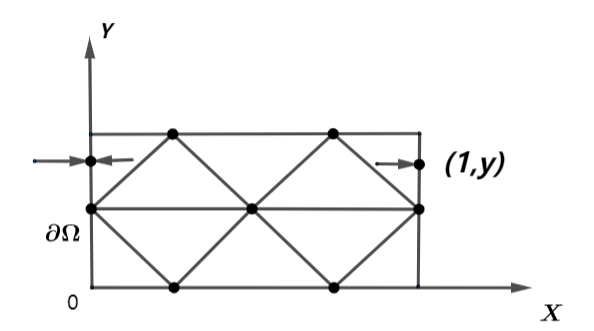
\includegraphics[width=0.4\textwidth]{images/6.png} 
	\caption{周期边界条件}
	\label{cycleboundary} 
\end{figure}
在左边界点 $(0, y)$处计算数值通量时,需要用到边界外侧的极限值 $\bs u_{h}^{\text{out}}(0, y, t)$,它由在点$(1, y)$处的单元内部的值 $\bs u_{h}^{\text{in}}(1, y, t)$ 给出。
\item 入流与出流边界:
$$ \bs u_{h}^{\text {out}}(x, y, t)=\bs u_{h}^{\text {in}}(x, y, t)$$

\item 反射边界:在反射边界处,密度$\rho$ 与能量 $E$取值大小相等,速度的法向分量大小相反,切向分量大小相等。
设向量 $\bs{n}=\left(n_{1}, n_{2}\right)$ 为单元K在$\partial\Omega$处的单位外法向量,切向量$\bs{\tau}=\left(-n_{2}, n_{1}\right)$有:
\begin{equation}
\begin{split}
&\begin{cases}
\rho^{\text{out}}=\rho^{\text {in}} \\
E^{\text {out}}=E^{\text {in}}
\end{cases},\quad
\begin{cases}
\left(\left(\rho \bs v_{1}\right)^{\text {out}},\left(\rho \bs v_{2}\right)^{\text {out}}\right) \cdot \bs{n}=\left(\left(\rho \bs v_{1}\right)^{\text{in}},\left(\rho \bs v_{2}\right)^{\text {in }}\right) \cdot(-\bs{n}) \\
\left(\left(\rho \bs v_{1}\right)^{\text{out}},\left(\rho \bs v_{2}\right)^{\text{out}}\right) \cdot \bs{\tau}=\left(\left(\rho \bs v_{1}\right)^{\text {in}},\left(\rho \bs v_{2}\right)^{\text {in }}\right) \cdot(\bs{\tau})	
\end{cases}\\
&\begin{bmatrix}
\left(\rho \bs v_{1}\right)^{\text {out}} \\
\left(\rho \bs v_{2}\right)^{\text {out}}
\end{bmatrix} = 
\begin{bmatrix}
n_{1} & -n_{2} \\
n_{2} & n_{1}
\end{bmatrix}
\begin{bmatrix}
-({\rho \bs{v}})^{\text{in }} \cdot \bs{n} \\
({\rho \bs{v}})^{\text {in }} \cdot \bs{\tau}
\end{bmatrix}
\end{split}
\end{equation}
\end{enumerate}

\begin{figure}[h] 
	\centering
	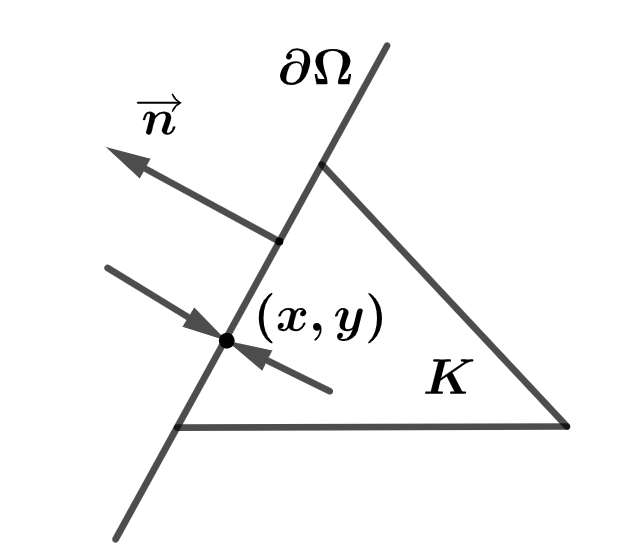
\includegraphics[width=0.3\textwidth]{images/7.png}
	\caption{入流与出流边界条件}  
	\label{inflowboundary}
\end{figure}

在处理边界条件时有两种方法:
\begin{itemize}
	\item 将靠近$\partial\Omega$的单元K沿着边界处翻转过来,设置一个虚拟单元K',进行编号。跟区域$\Omega$内部的单元K一样,在K'上定义数值解。这样做的好处是:计算数值通量时,在区域$\Omega$的内部单元与边界单元处可以统一处理。
	
	\item 不设置虚拟单元,在区域边界$\partial\Omega$处计算数值通量时需用到数值解在边界外侧的极限值,它可以由边界条件直接给出。
\end{itemize}

\end{document}